\section{\achswlm for Hierarchical Classification}
Two\:-\:dimensional separability as the main properties of \achswlm makes the learned representations of the entities in the hierarchy less sensitive to the structural changes for instance when the hierarchy evolves over time. Here in this section, we address our last research question of this chapter:
\begin{resqbox}
\emph{\resq{c3.3}}
\end{resqbox}

Before evaluating the the transferability of of two\:-\:dimensionaly separable representations over time, we intrinsically study the separability of the representations learned by \achswlm. We use parliamentary data as one of the interesting collections with hierarchically structured data that can evolve over time. The structure of the parliamentary hierarchy has been shown in Figure~\ref{fig:ParHierarchy}.  First, we introduce the collection we have used, and then we analyze the quality of \achswlm on providing horizontal and vertical separability over the hierarchy. 

\subsection{Data Collection}
We use the Dutch parliamentary data which forms a hierarchical structure that can evolve over time. The data are collected and annotated as the part of
\emph{Political\-Mashup} project \citep{url:politicalmashup} to make semantically enriched parliamentary proceedings available as open data \citep{marx:2010}.

As a brief background, the Dutch parliament is a bicameral parliament which consists of the Senate and the house of representatives. The house of representatives is the main chamber of parliament, where discussion of proposed legislation and review of the government's actions takes place.  The Dutch parliamentary system is a multi-party system, requiring a coalition of parties to form the government~\citep{deswaan73}.

\begin{figure*}[!t]
\centering
\makebox[\linewidth][c]{
\resizebox{\linewidth}{!}{%
\tikzset{
every tree node/.style={align=center,anchor=north}
edge from parent/.style={very thick},
%edge from parent/.style=
%{draw, edge from parent path={(\tikzparentnode.south)
%-- +(0,-8pt)
%-| (\tikzchildnode)}},
blank/.style={draw=none}}
\begin{tikzpicture}[level distance = 30pt]
\fontsize{7}{8}\selectfont{
\matrix (magic) [ampersand replacement=\&]
{
\node{\Tree
    [.All  \edge[blank]; 
    [.Status  \edge[blank];
    [.Party \edge[blank]; 
    [.Mem\# ]]]]};
\&
\node{
    \Tree 
    [.\small{Parliament(2006-2010)}
        [.Government 
            [.$CDA$  $47$ ]
            [.$PvdA$  $37$ ]
            [.$CU$  $6$ ]
        ]
        [.Opposition 
            [.$VVD$  $24$ ]
            [.$PVV$  $10$ ]
            [.$SP$  $27$ ]
            [.$D66$  $3$ ]
            [.$GL$  $10$ ]
        ]
    ]};
\&
\node{
    \Tree 
    [.\small{Parliament(2010-2012)}
        [.Government 
            [.$VVD$  $33$ ]
            [.$CDA$  $23$ ]
        ]
        [.Oppositions
            [.$PvdA$  $32$ ]
            [.$PVV$  $22$ ]
            [.$SP$  $16$ ]
            [.$D66$  $10$ ]
            [.$CU$  $6$ ]
            [.$GL$  $12$ ]
        ]
    ]};
\&
\node{
    \Tree 
    [.\small{Parliament(2012-2014)}
        [.Government 
            [.$VVD$  $43$ ]
            [.$PvdA$  $42$ ]
        ]
        [.Opposition 
            [.$CDA$  $13$ ]
            [.$PVV$  $12$ ]
            [.$SP$  $18$ ]
            [.$D66$  $12$ ]
            [.$CU$  $5$ ]
            [.$GL$  $4$ ]
        ]
    ]};\\
};
}
\end{tikzpicture}
}
}
\caption{Composition of Dutch parliament in 3 periods. \emph{VVD}:People's Party for Freedom and democracy, \emph{PvdA}:Labour Party, \emph{CDA}:Christian Democratic Appeal, \emph{PVV}:Party for Freedom, \emph{SP}:The Socialist Party, \emph{D66}:Democrats 66, \emph{GL}:Green-Left, \emph{CU}:Christian-Union.}
\label{fig:DutchParl}
\end{figure*}
We use data from the parliament or the House of Representatives of the Netherlands.  We have chosen three interesting periods of parliament, from March 2006 to April 2014, in which eight main parties have about 95\% of seats in the parliament: People's Party for Freedom and Democracy, Labour Party, Christian Democratic Appeal, Party for Freedom, The Socialist Party, Democrats 66, Green-Left, Christian-Union.   The coalition in the first period is between a left-wing party and a centrist party, in the second period between a right-wing party and centrism party, and in the third, between a right-wing and left-wing party. Figure~\ref{fig:DutchParl} shows the hierarchical structure of the Dutch parliament in these three different periods.

In order to learn representations for parliamentary entities, first of all,  we prepare the data. In the proceedings, there are series of parliamentary speeches by different MPs following the debate structure.  We invert the data matrix so that for each speaker we collect their speeches as a single document that reflects the features of that member. Then, for representing the internal entities in the parliament's hierarchy, we first consider members as the leaf entities and then concatenate all leaf documents below internal entities as a single document which textually represents them: first over parties, and then parties into government and opposition, etc.
%
The whole corpus consists of 14.7 million terms from 240,501 speeches and contains 2.1 million unique terms. 
No stemming and no lemmatization is done on the data and also stop words, and common words are not removed in data preprocessing.  After data preparation, we estimate \acswlm\ for all entities in the hierarchy as it is explained in Section~\ref{sec:hswlm}.

%---------------------------------------
\sshrink
\subsection{Two\:-\:Dimensional Separability of \achswlm}
\label{subsec:achswlmep}
%---------------------------------------
Here we investigate the ability of \achswlm on providing language models for hierarchical entities that are two\:-\:dimensionally separable. 
Based on the explained procedure of estimating \achswlm, the language models of entities in the hierarchy is repeatedly updated, so that the resulting models are both \emph{horizontally} and \emph{vertically} separable in the hierarchy. To assess this fact, we estimate \achswlm on the parliamentary data and look into the separability between entities in the same layer or in different layers.

Figures~\ref{fig:HSS} and~\ref{fig:HSP} illustrate the probability distribution over terms based on the estimated \achswlm in the status and party layer respectively. We sort the probability distribution on the term weight of the first model and plot the other models in this exact order.
As can be seen in the status layer, Figures~\ref{fig:HSS}, the distributions over terms for government and opposition cover almost separated set of terms. Since in this layer these two entities are supposed to be against each other, a high level of separability can be expected. On the other hand, in the party layer, Figures \ref{fig:HSP}, it is possible that two parties share some ideological issues and consequently share some terms. So, in this layer, a complete separability of terms would not be practically possible for all the parties. Nevertheless, \achswlm provides an acceptable horizontal separability in this layer.


\begin{figure}[t]
    \centering
    \begin{subfigure}[b]{0.32\textwidth}
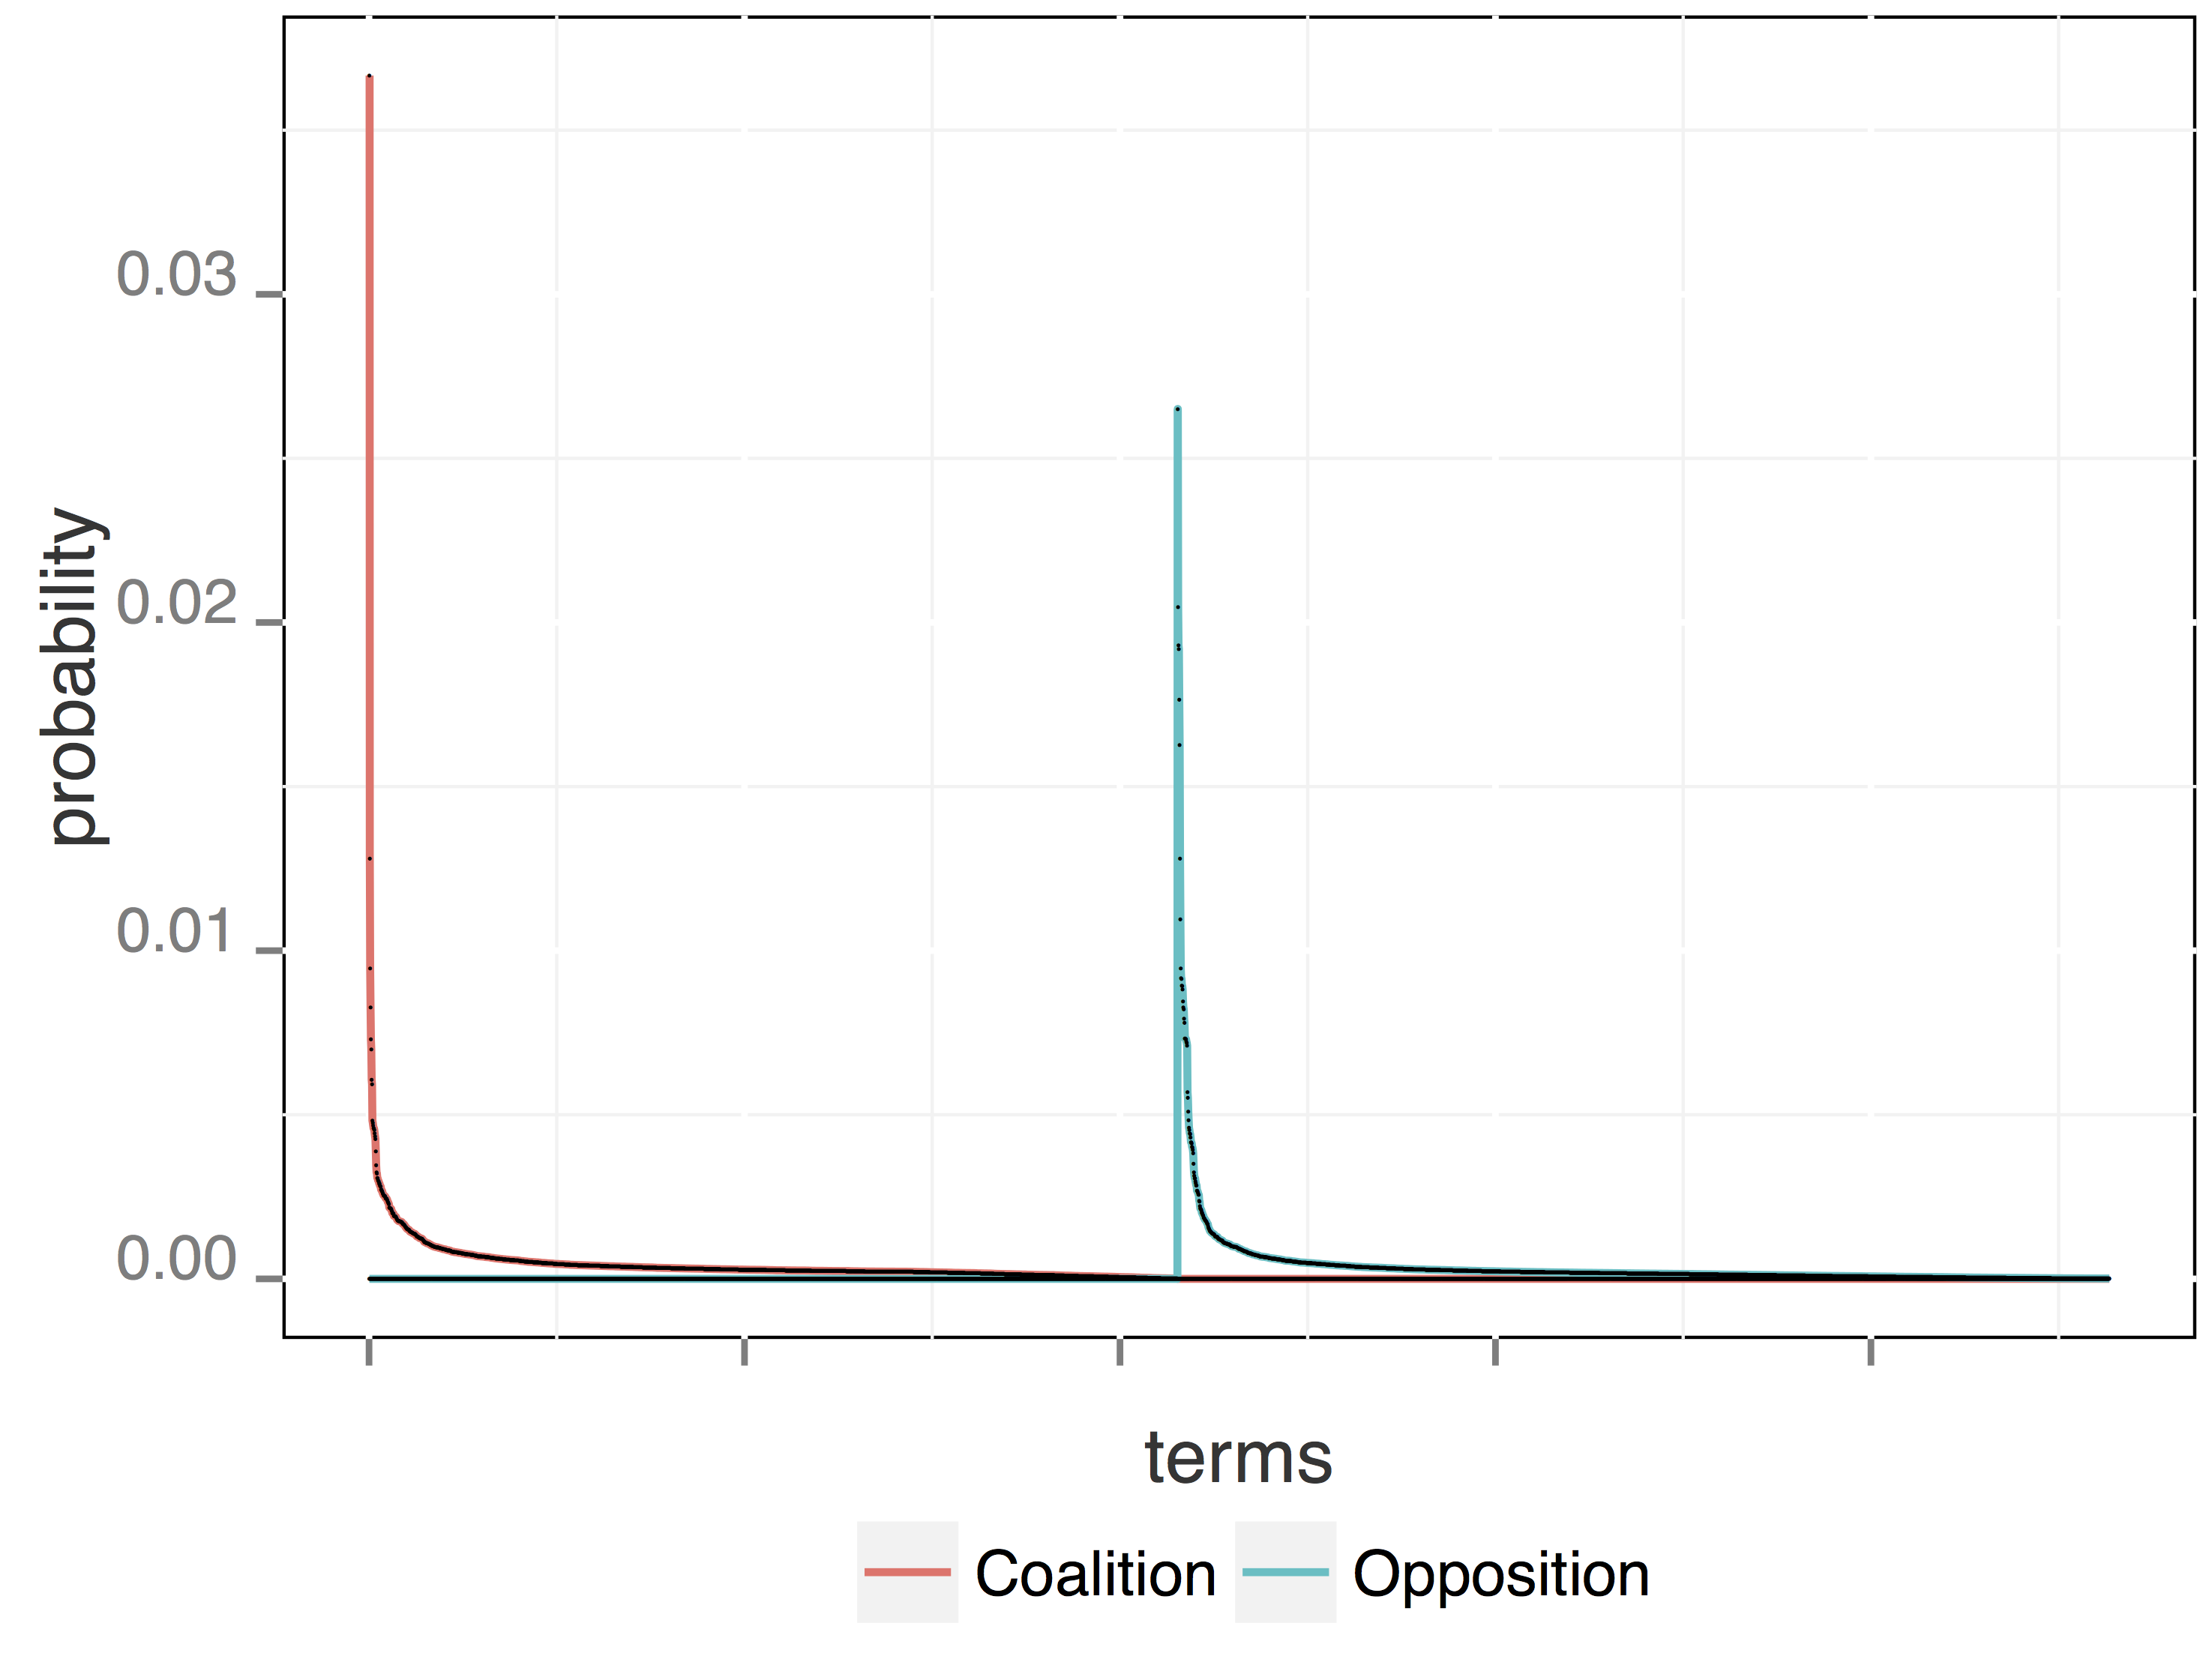
\includegraphics[width=\linewidth]{02-part-01/chapter-03/figs_and_tables/img_opo-coa.png}
\caption{\label{fig:HSS}\achswlm in the status layer}
        \end{subfigure}
        ~ 
    \begin{subfigure}[b]{0.64\textwidth}
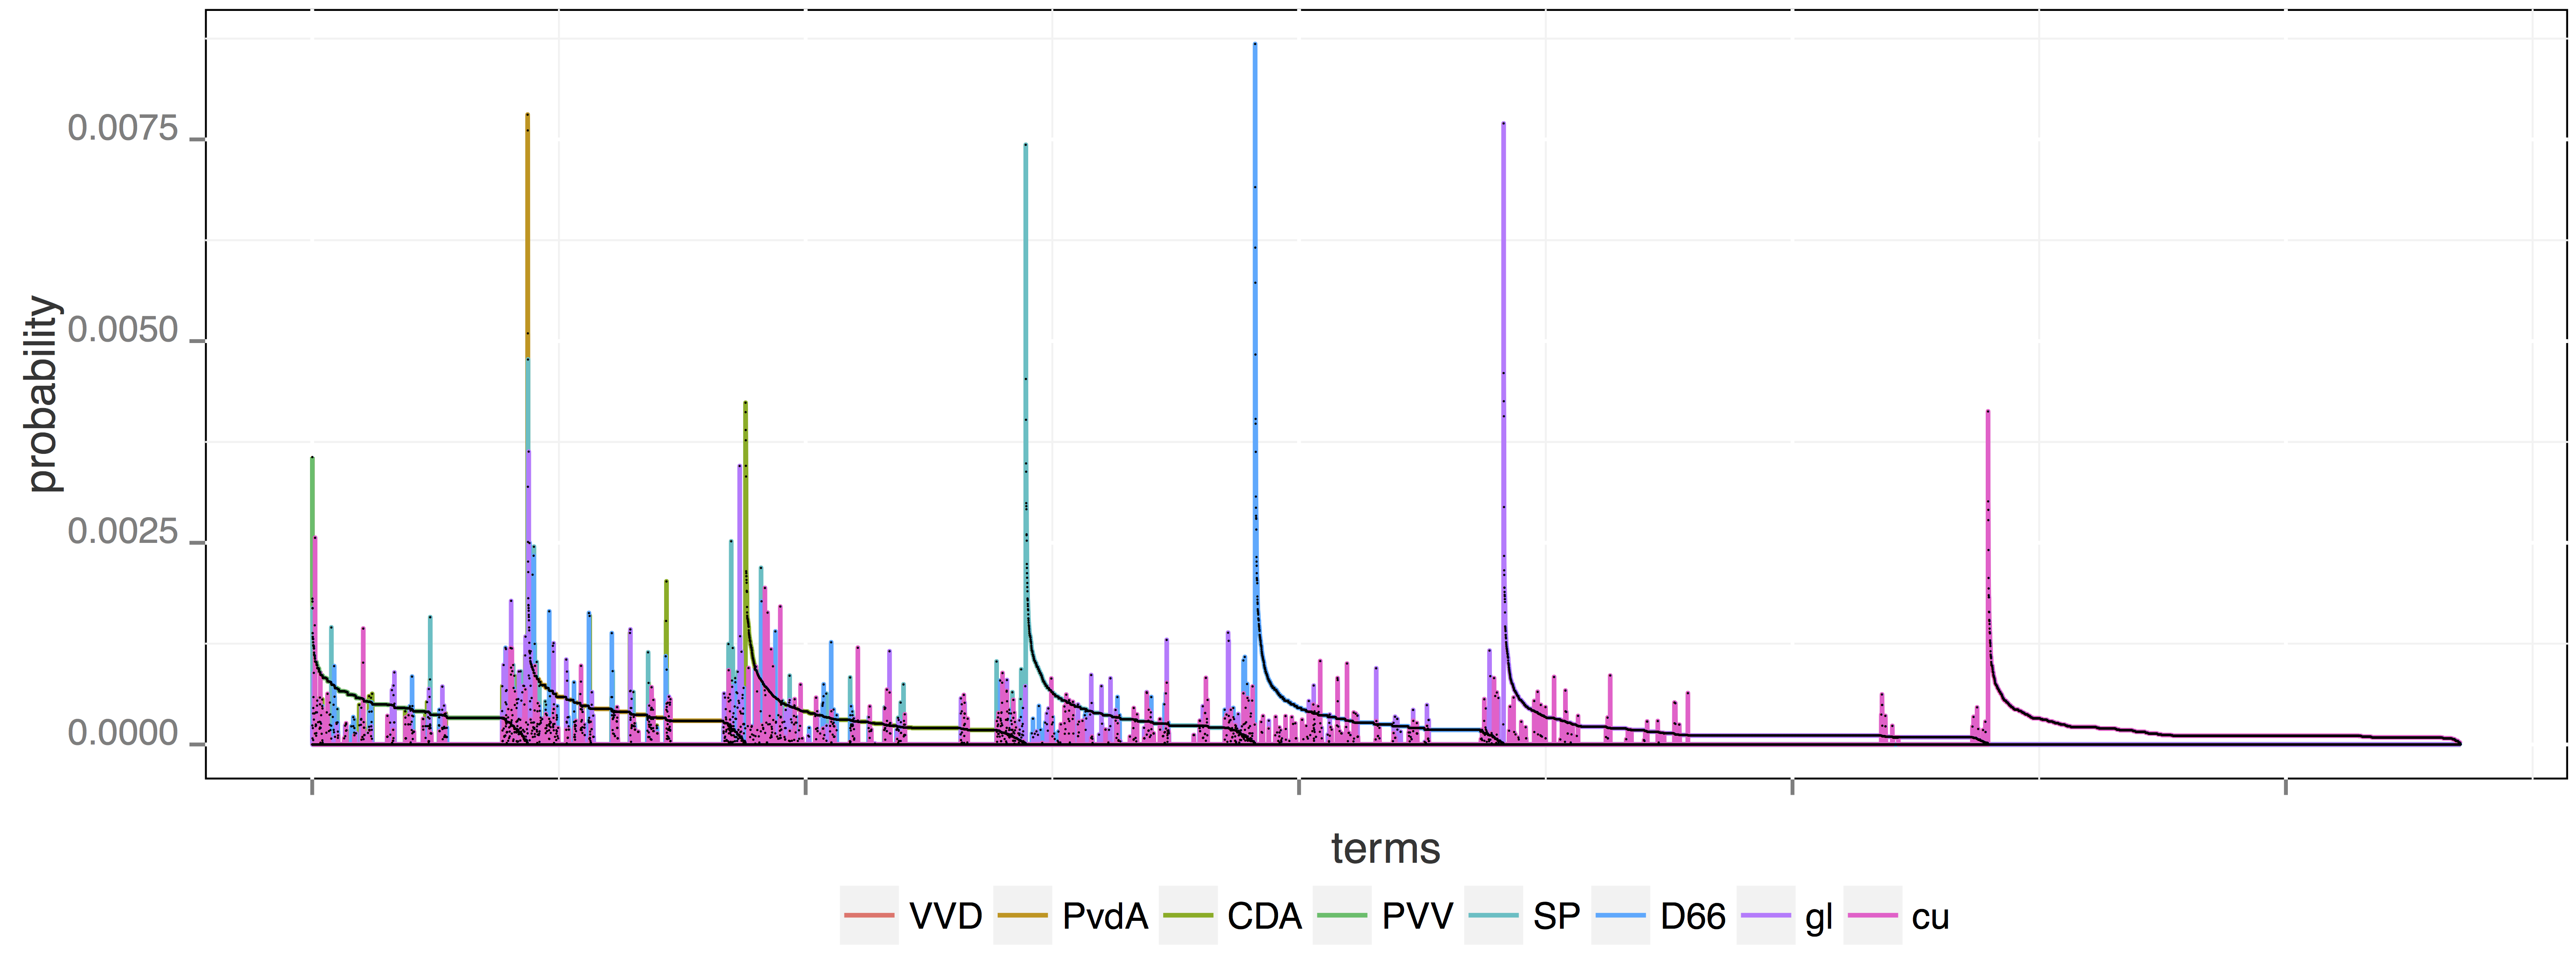
\includegraphics[width=\linewidth]{02-part-01/chapter-03/figs_and_tables/img_parties.png}
\caption{\label{fig:HSP}\achswlm in the party layer}
        \end{subfigure}
    \caption{\label{fig:HS} \emph{Horizontal Separability}: probability distribution over terms based on \hswlms in status layer and party layer.}
\end{figure}

Besides, we illustrate the horizontal separability of \achswlm of some pairs of parties. Figures \ref{fig:HSPCO}, \ref{fig:HSPOO}, and \ref{fig:HSPCC} show the separability of models of two parties in three cases, respectively: 1) different statuses, 2) both in the status of opposition, 3) both in the status of government. It can be seen that in all cases of being in the same status or different status, estimated \hswlms are separable. The interesting point is in Figure~\ref{fig:HSPCC} that presents the models of two government parties that are strongly separable. This rooted in the fact that in this period there was an unusual coalition government consisting of a right\:-\:wing and a left\:-\:wing party. So, although they have agreement in the status layer, their model is highly separable in terms of having opposite spectrum in party layer.


\begin{figure}[!t]
        \centering
        \begin{subfigure}[b]{0.32\textwidth}
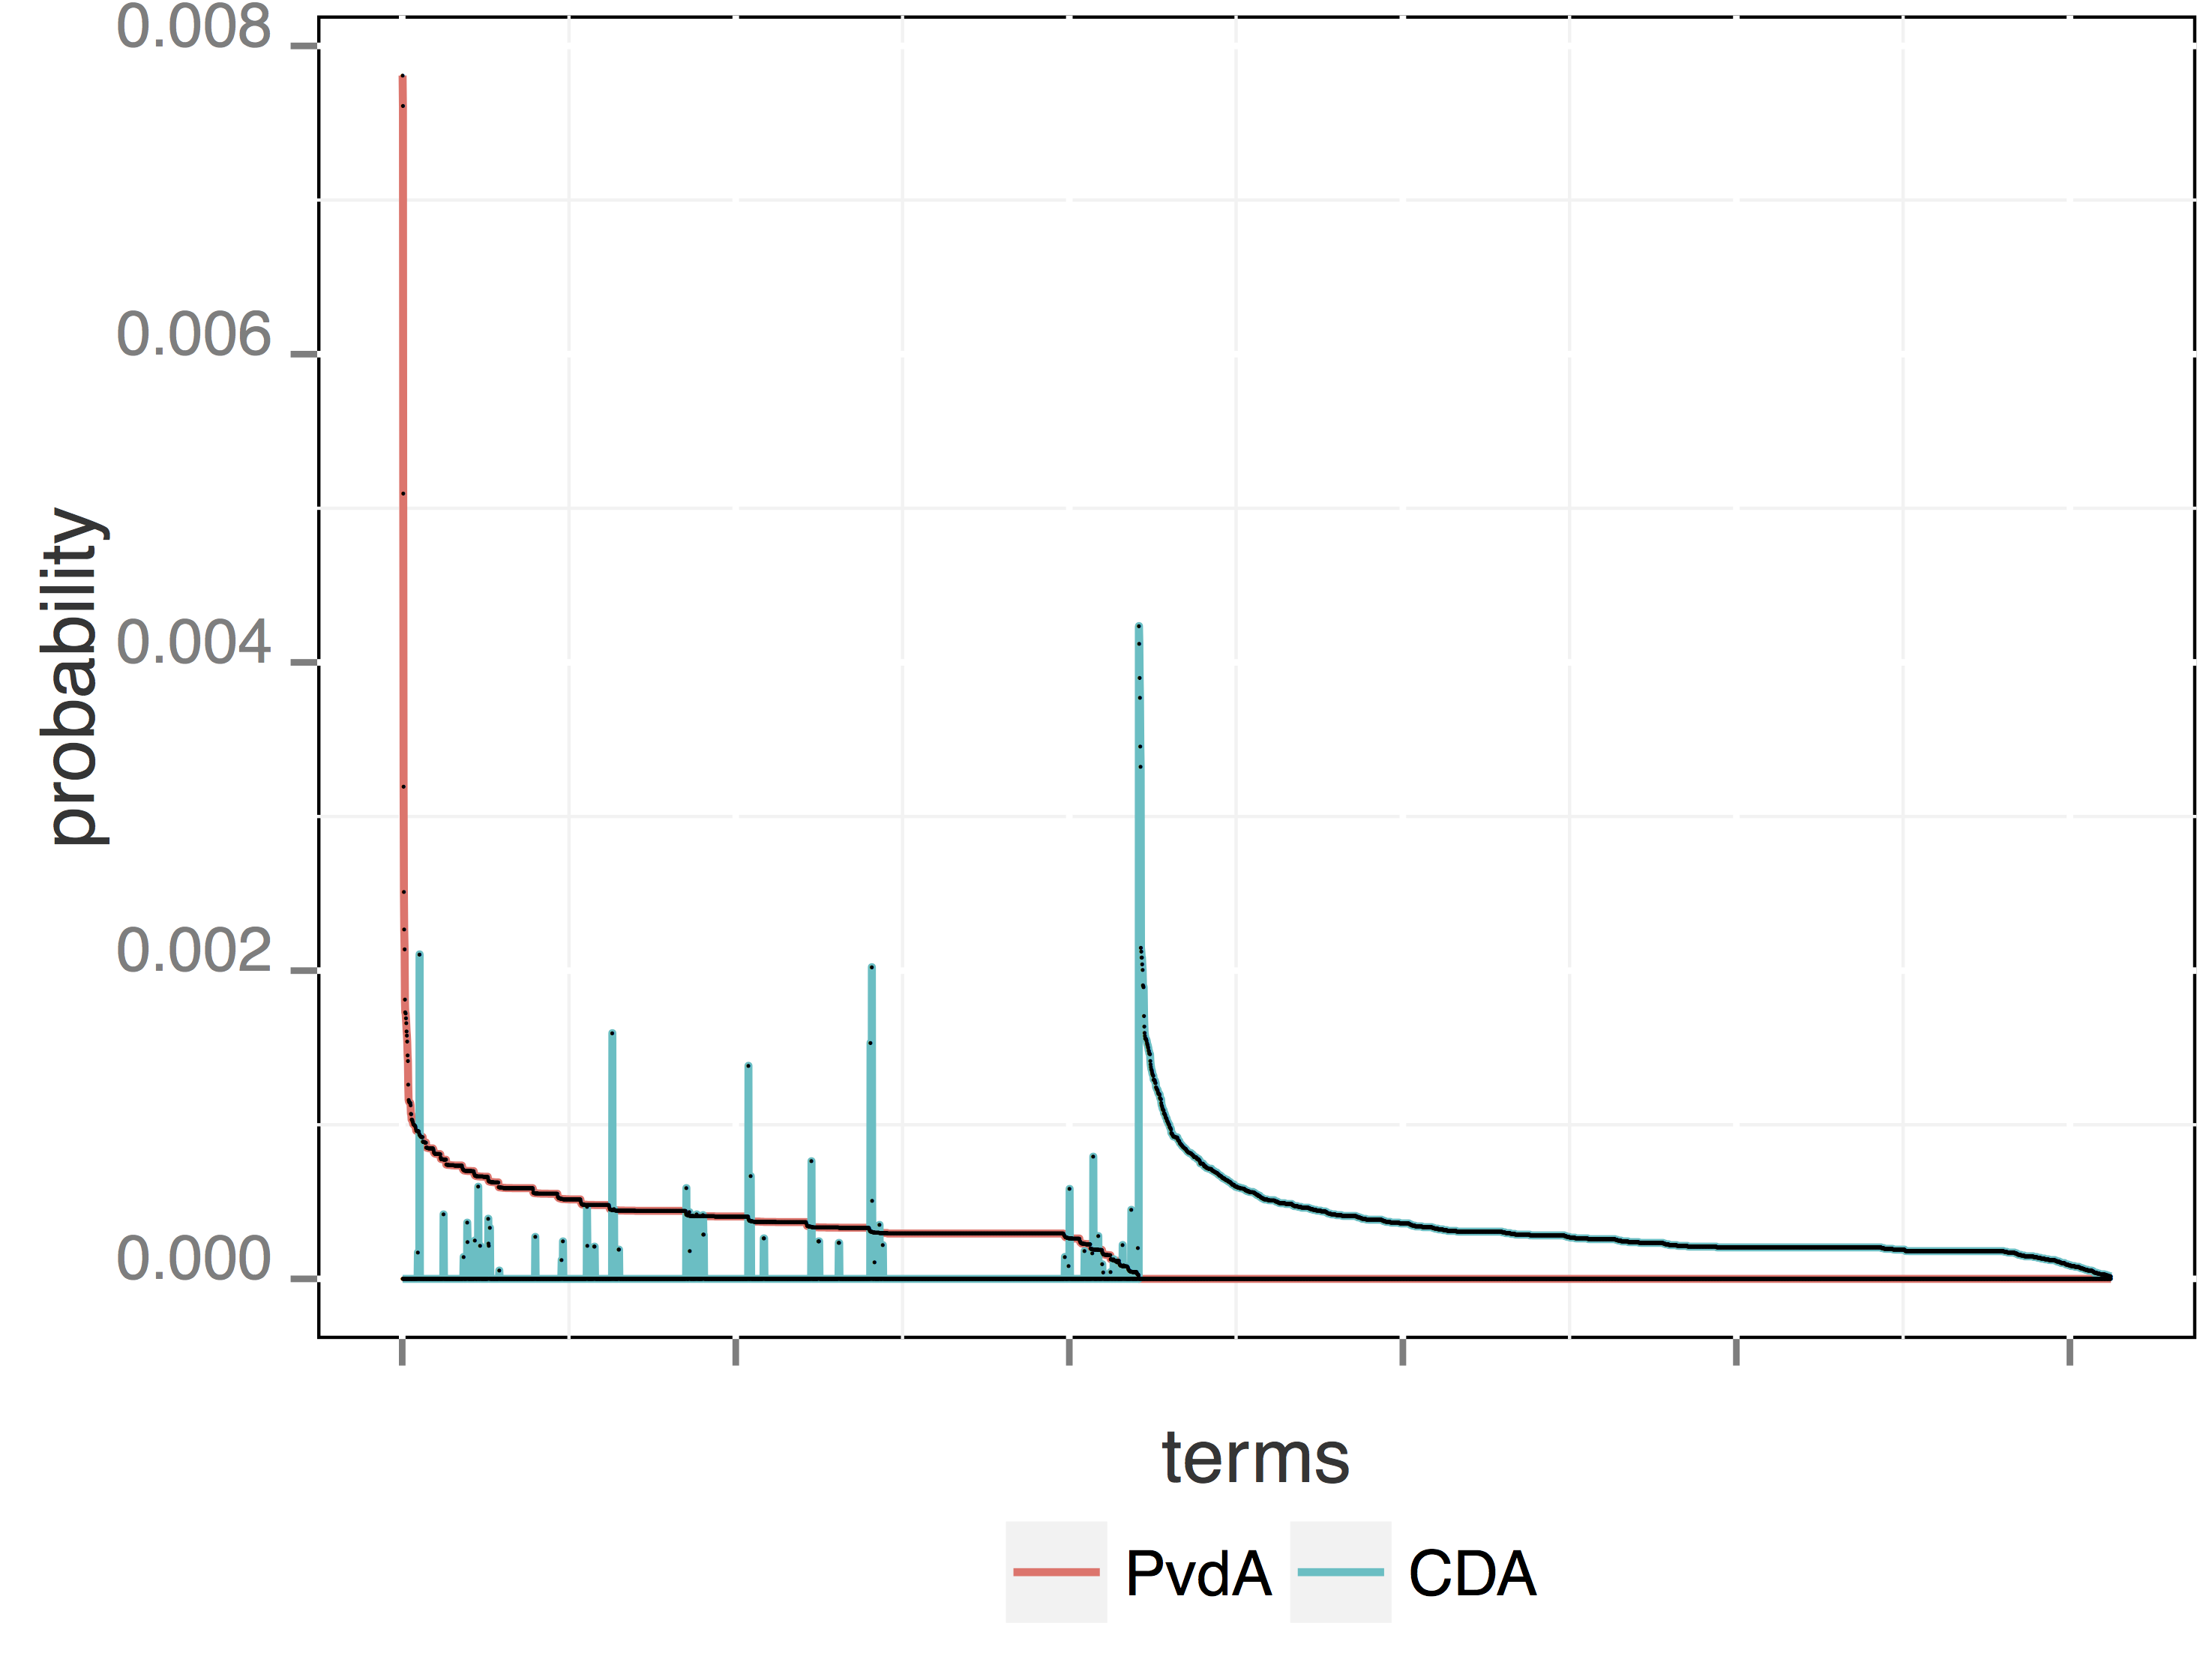
\includegraphics[width=\linewidth]{02-part-01/chapter-03/figs_and_tables/img_PvdA-CDA.png}
\caption{\label{fig:HSPCO} \achswlm of two parties in different statuses: Christian Democratic Appeal (CDA) and Labour Party (PvdA)}
        \end{subfigure}
        ~ 
        \begin{subfigure}[b]{0.32\textwidth}
\centering
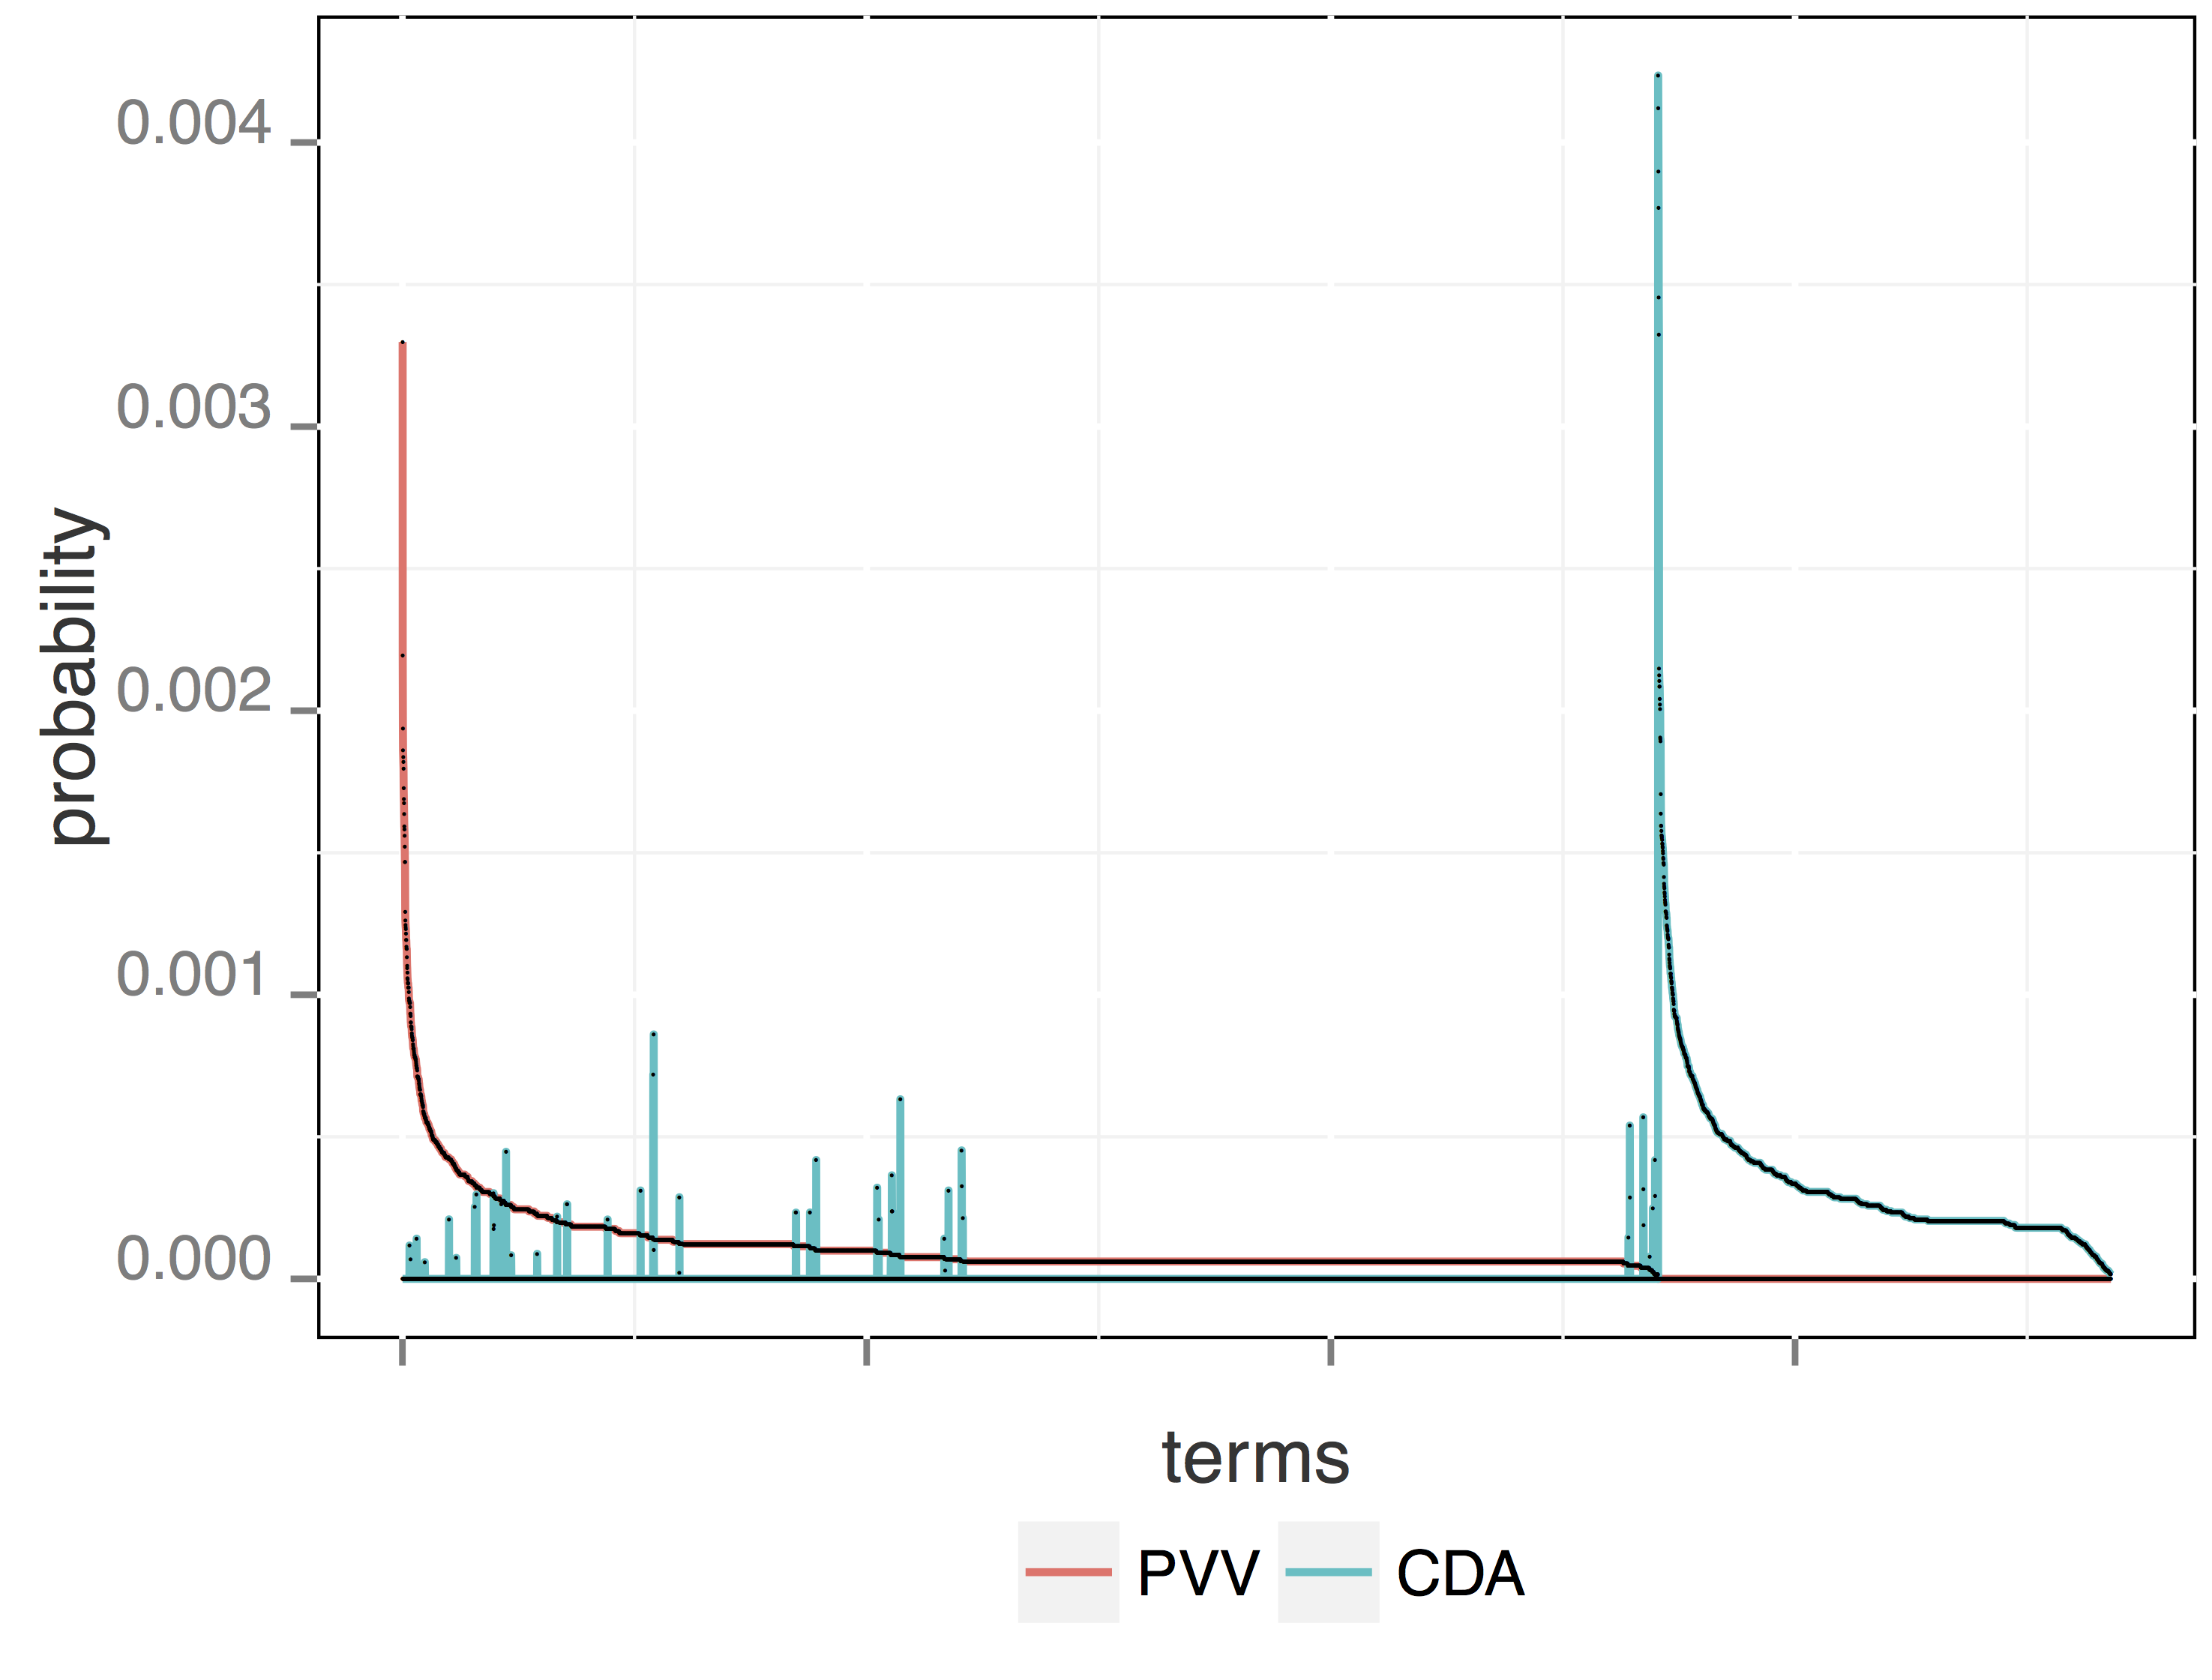
\includegraphics[width=\linewidth]{02-part-01/chapter-03/figs_and_tables/img_PVV-CDA.png}
\caption{\label{fig:HSPOO} \achswlm of two parties in opposition: Party for Freedom (PVV) and Christian Democratic Appeal (CDA)}
        \end{subfigure}
        ~ 
        \begin{subfigure}[b]{0.32\textwidth}
\centering
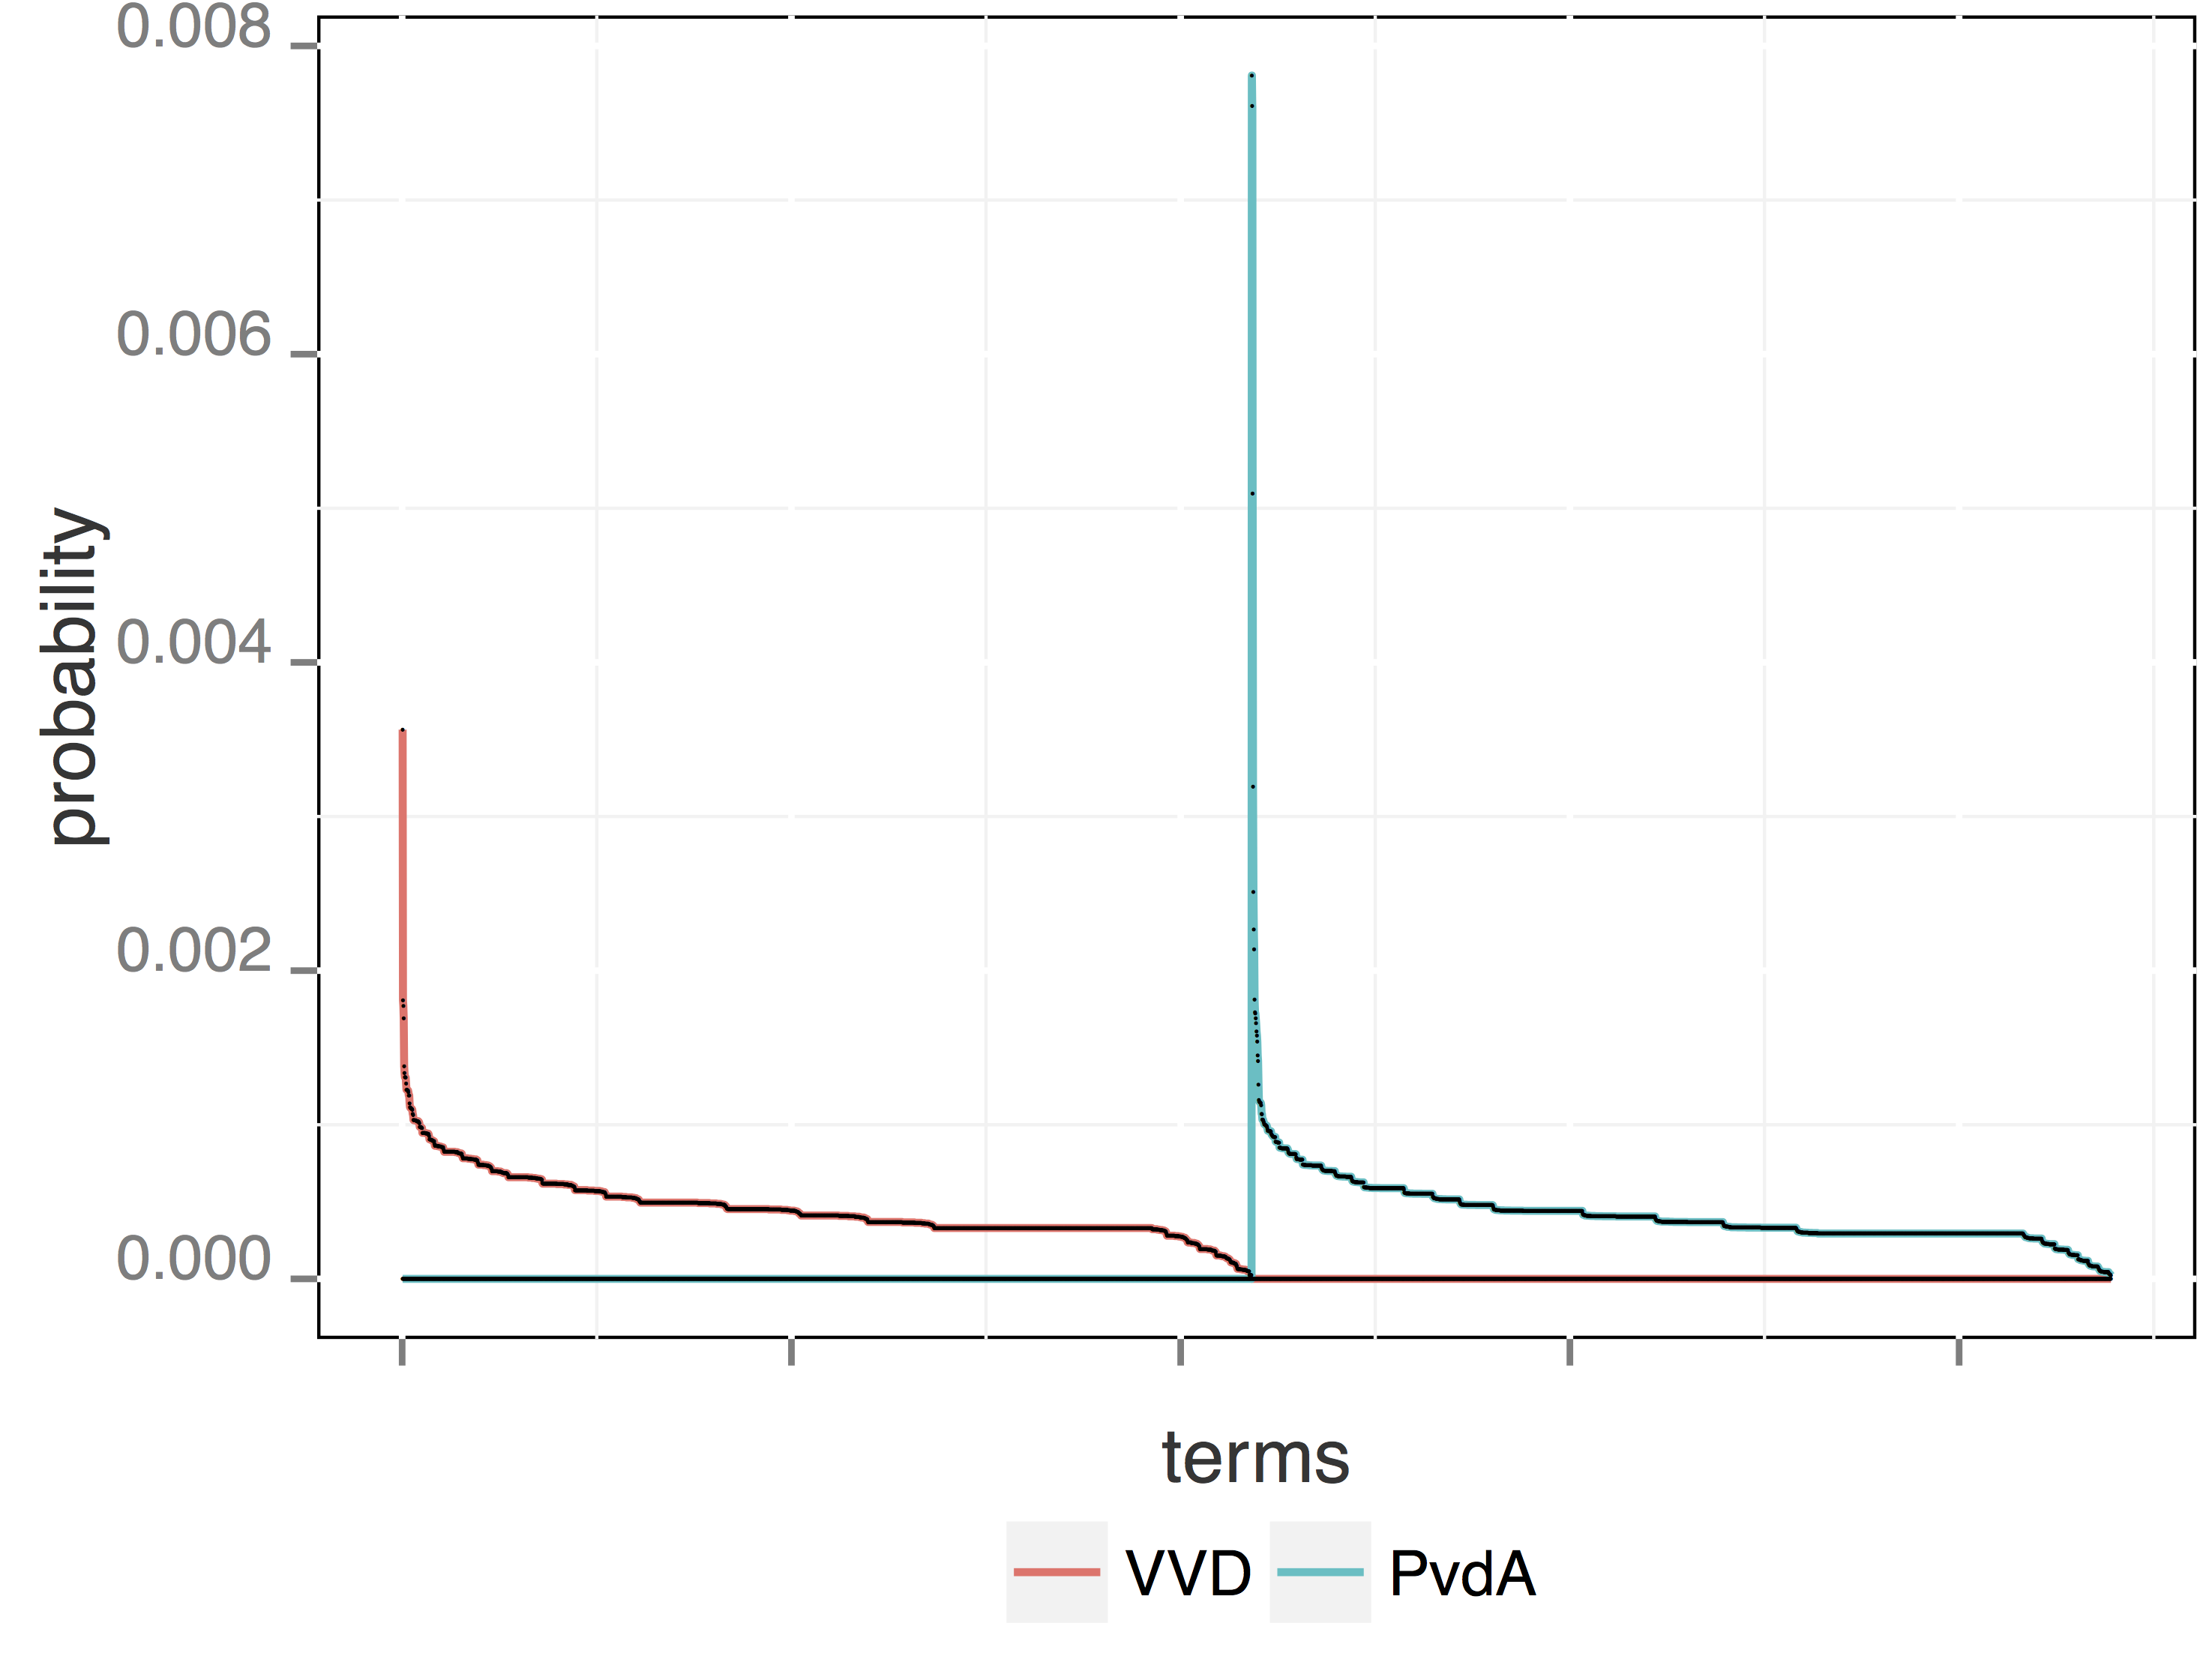
\includegraphics[width=\linewidth]{02-part-01/chapter-03/figs_and_tables/img_VVD-PvdA.png}
\caption{\label{fig:HSPCC} \achswlm of two parties in government: People's Party for Freedom (VVD) and Labour Party (PvdA)}
        \end{subfigure}
        \caption{\label{fig:HSP-pairs} \emph{Horizontal Separability}: probability distribution over terms based on \hswlms in party layer}
\end{figure}

In order to illustrate the vertical separability of \achswlm, we choose two different branches in the hierarchy: one from the leader of one of the opposition parties to the root, and the other from the leader of one of the government parties to the root. Figures \ref{fig:VSO} and \ref{fig:VSC} show probability distributions over words based on \achswlm of all entities in these two branches. They demonstrate that using \achswlm, we can decompose distribution over all terms to the highly separable distributions, each one representing the language usage related to the meaning behind the layer of the entity in the hierarchy. 

\begin{figure}[!t]
        \centering
        \begin{subfigure}[b]{0.45\textwidth}
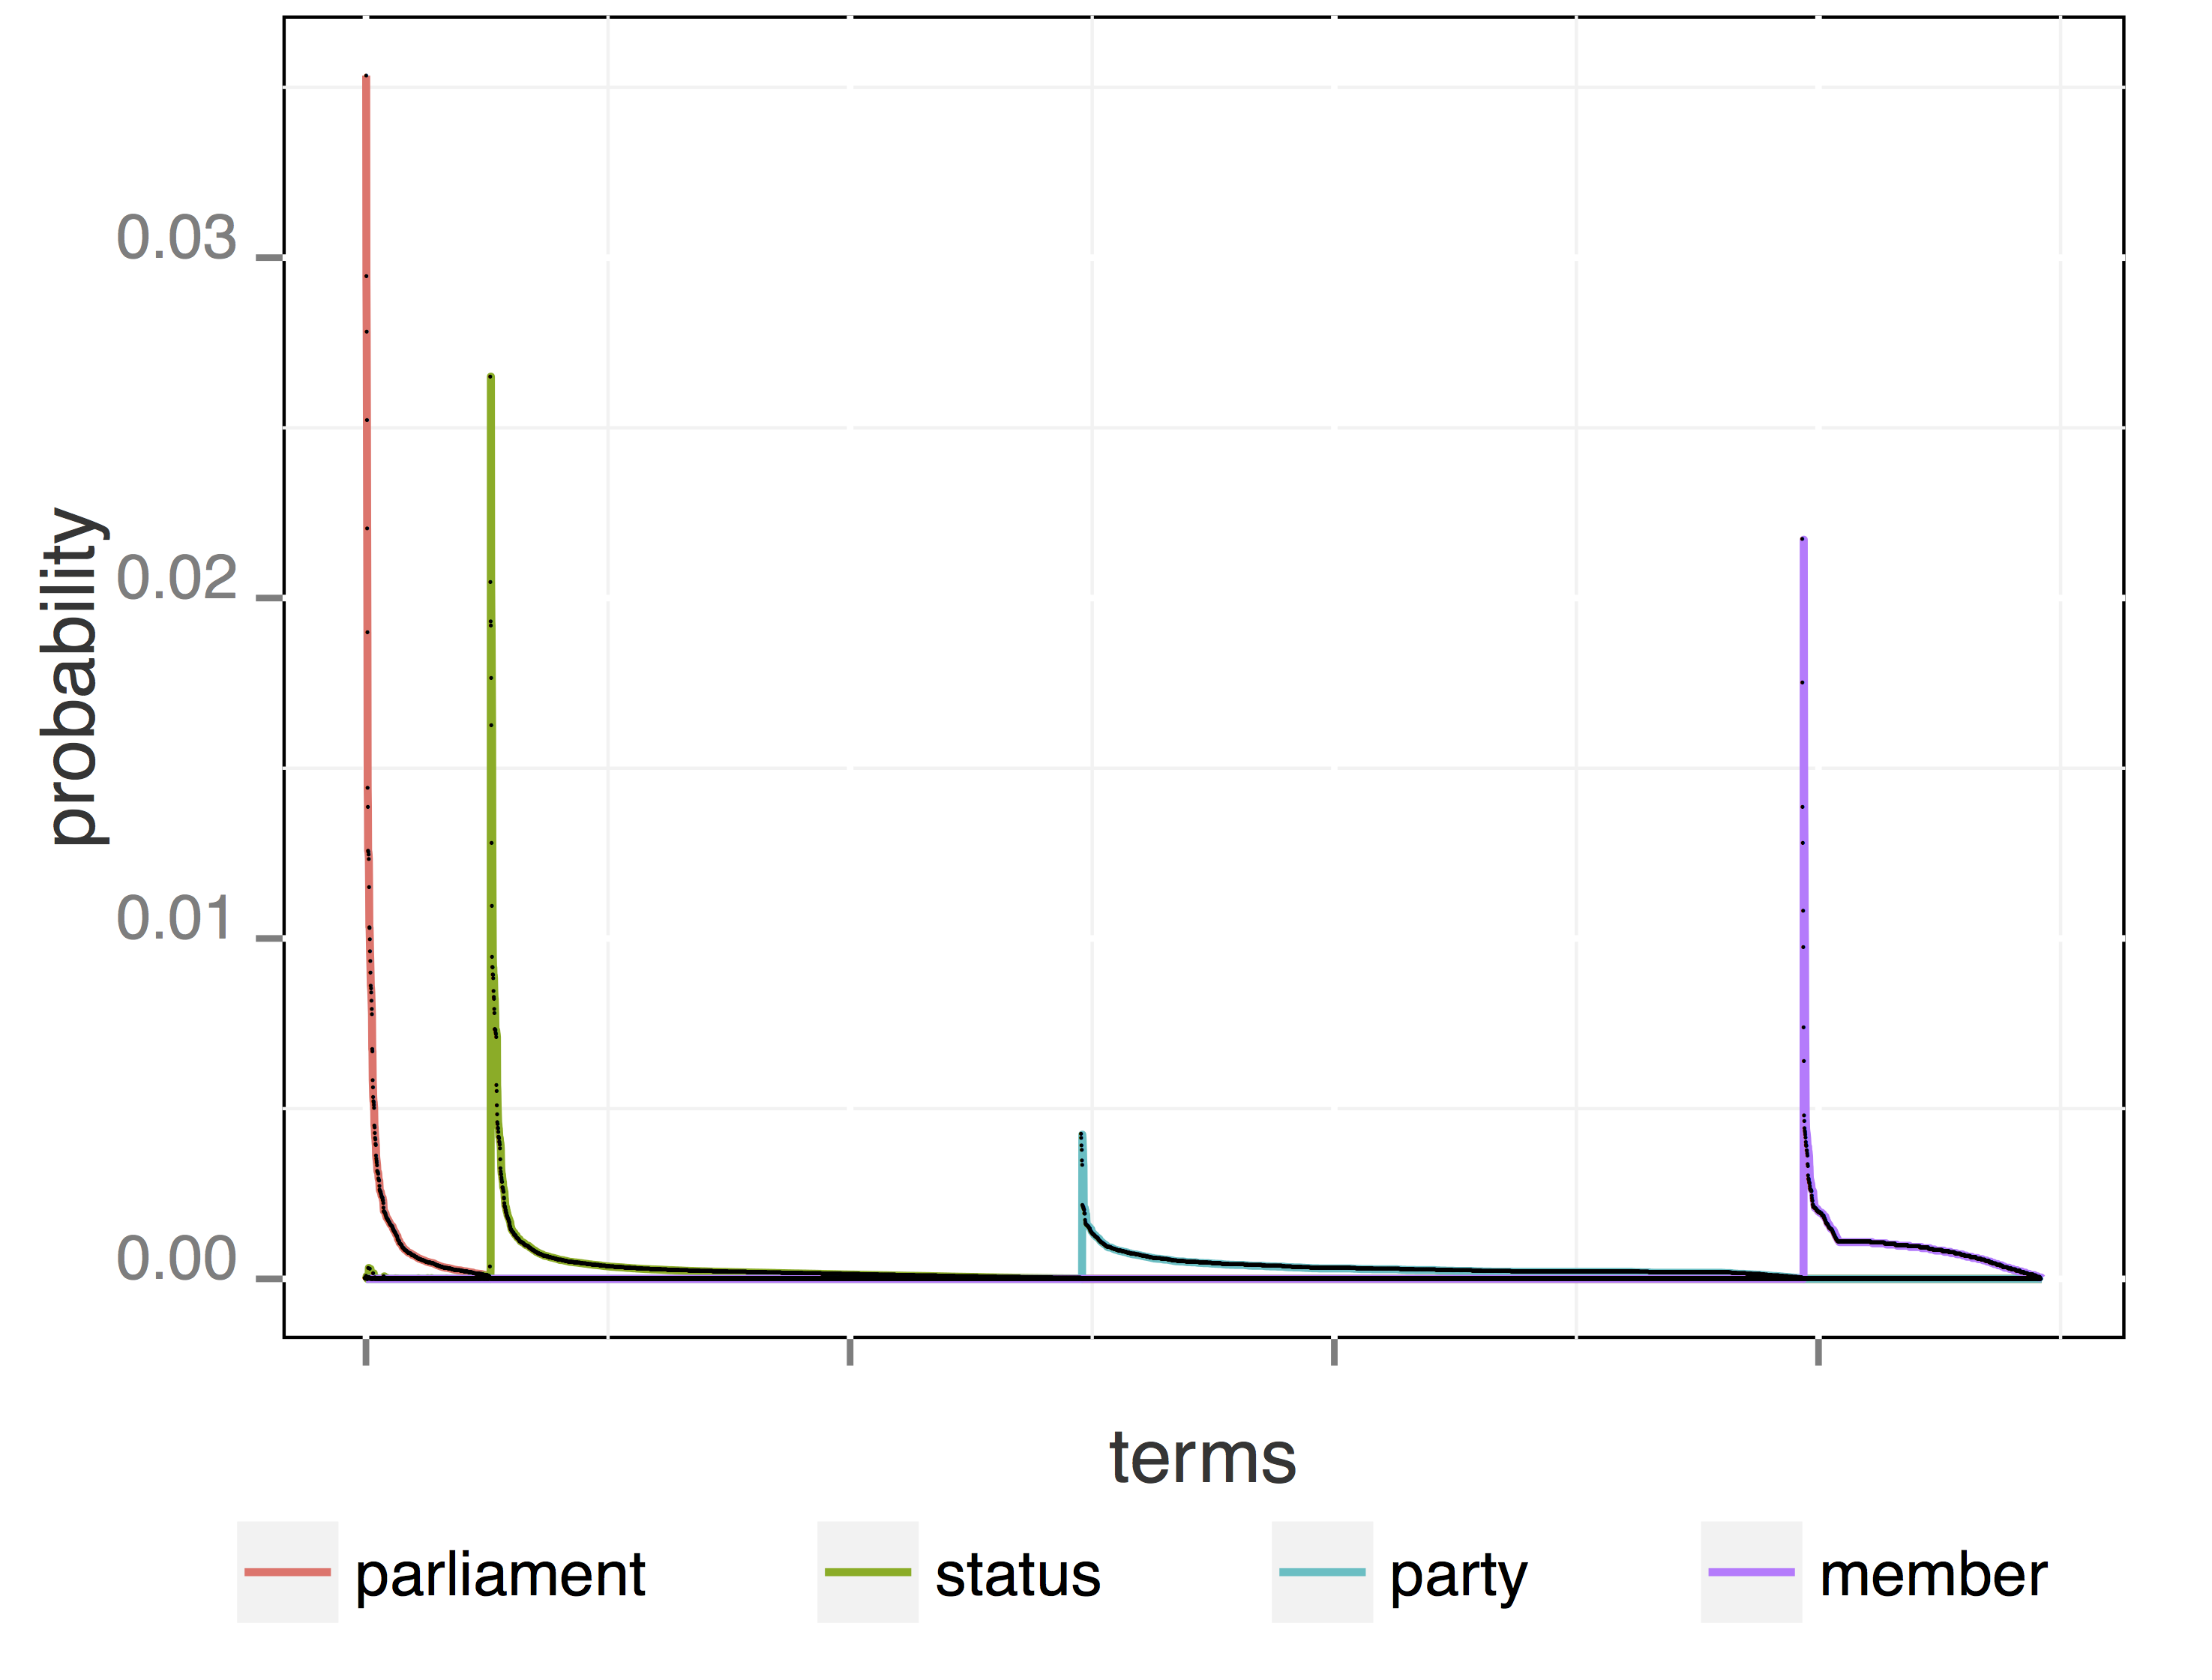
\includegraphics[width=\linewidth]{02-part-01/chapter-03/figs_and_tables/img_nlm02316.png}
\caption{\label{fig:VSO} \achswlm of S. van Haersma Buma (as the member of parliament - Leader of CDA), Christian Democratic Appeal (as the party), Opposition (as the status), and the Parliament}
        \end{subfigure}
        ~~~~~~~~
        \begin{subfigure}[b]{0.45\textwidth}
\centering
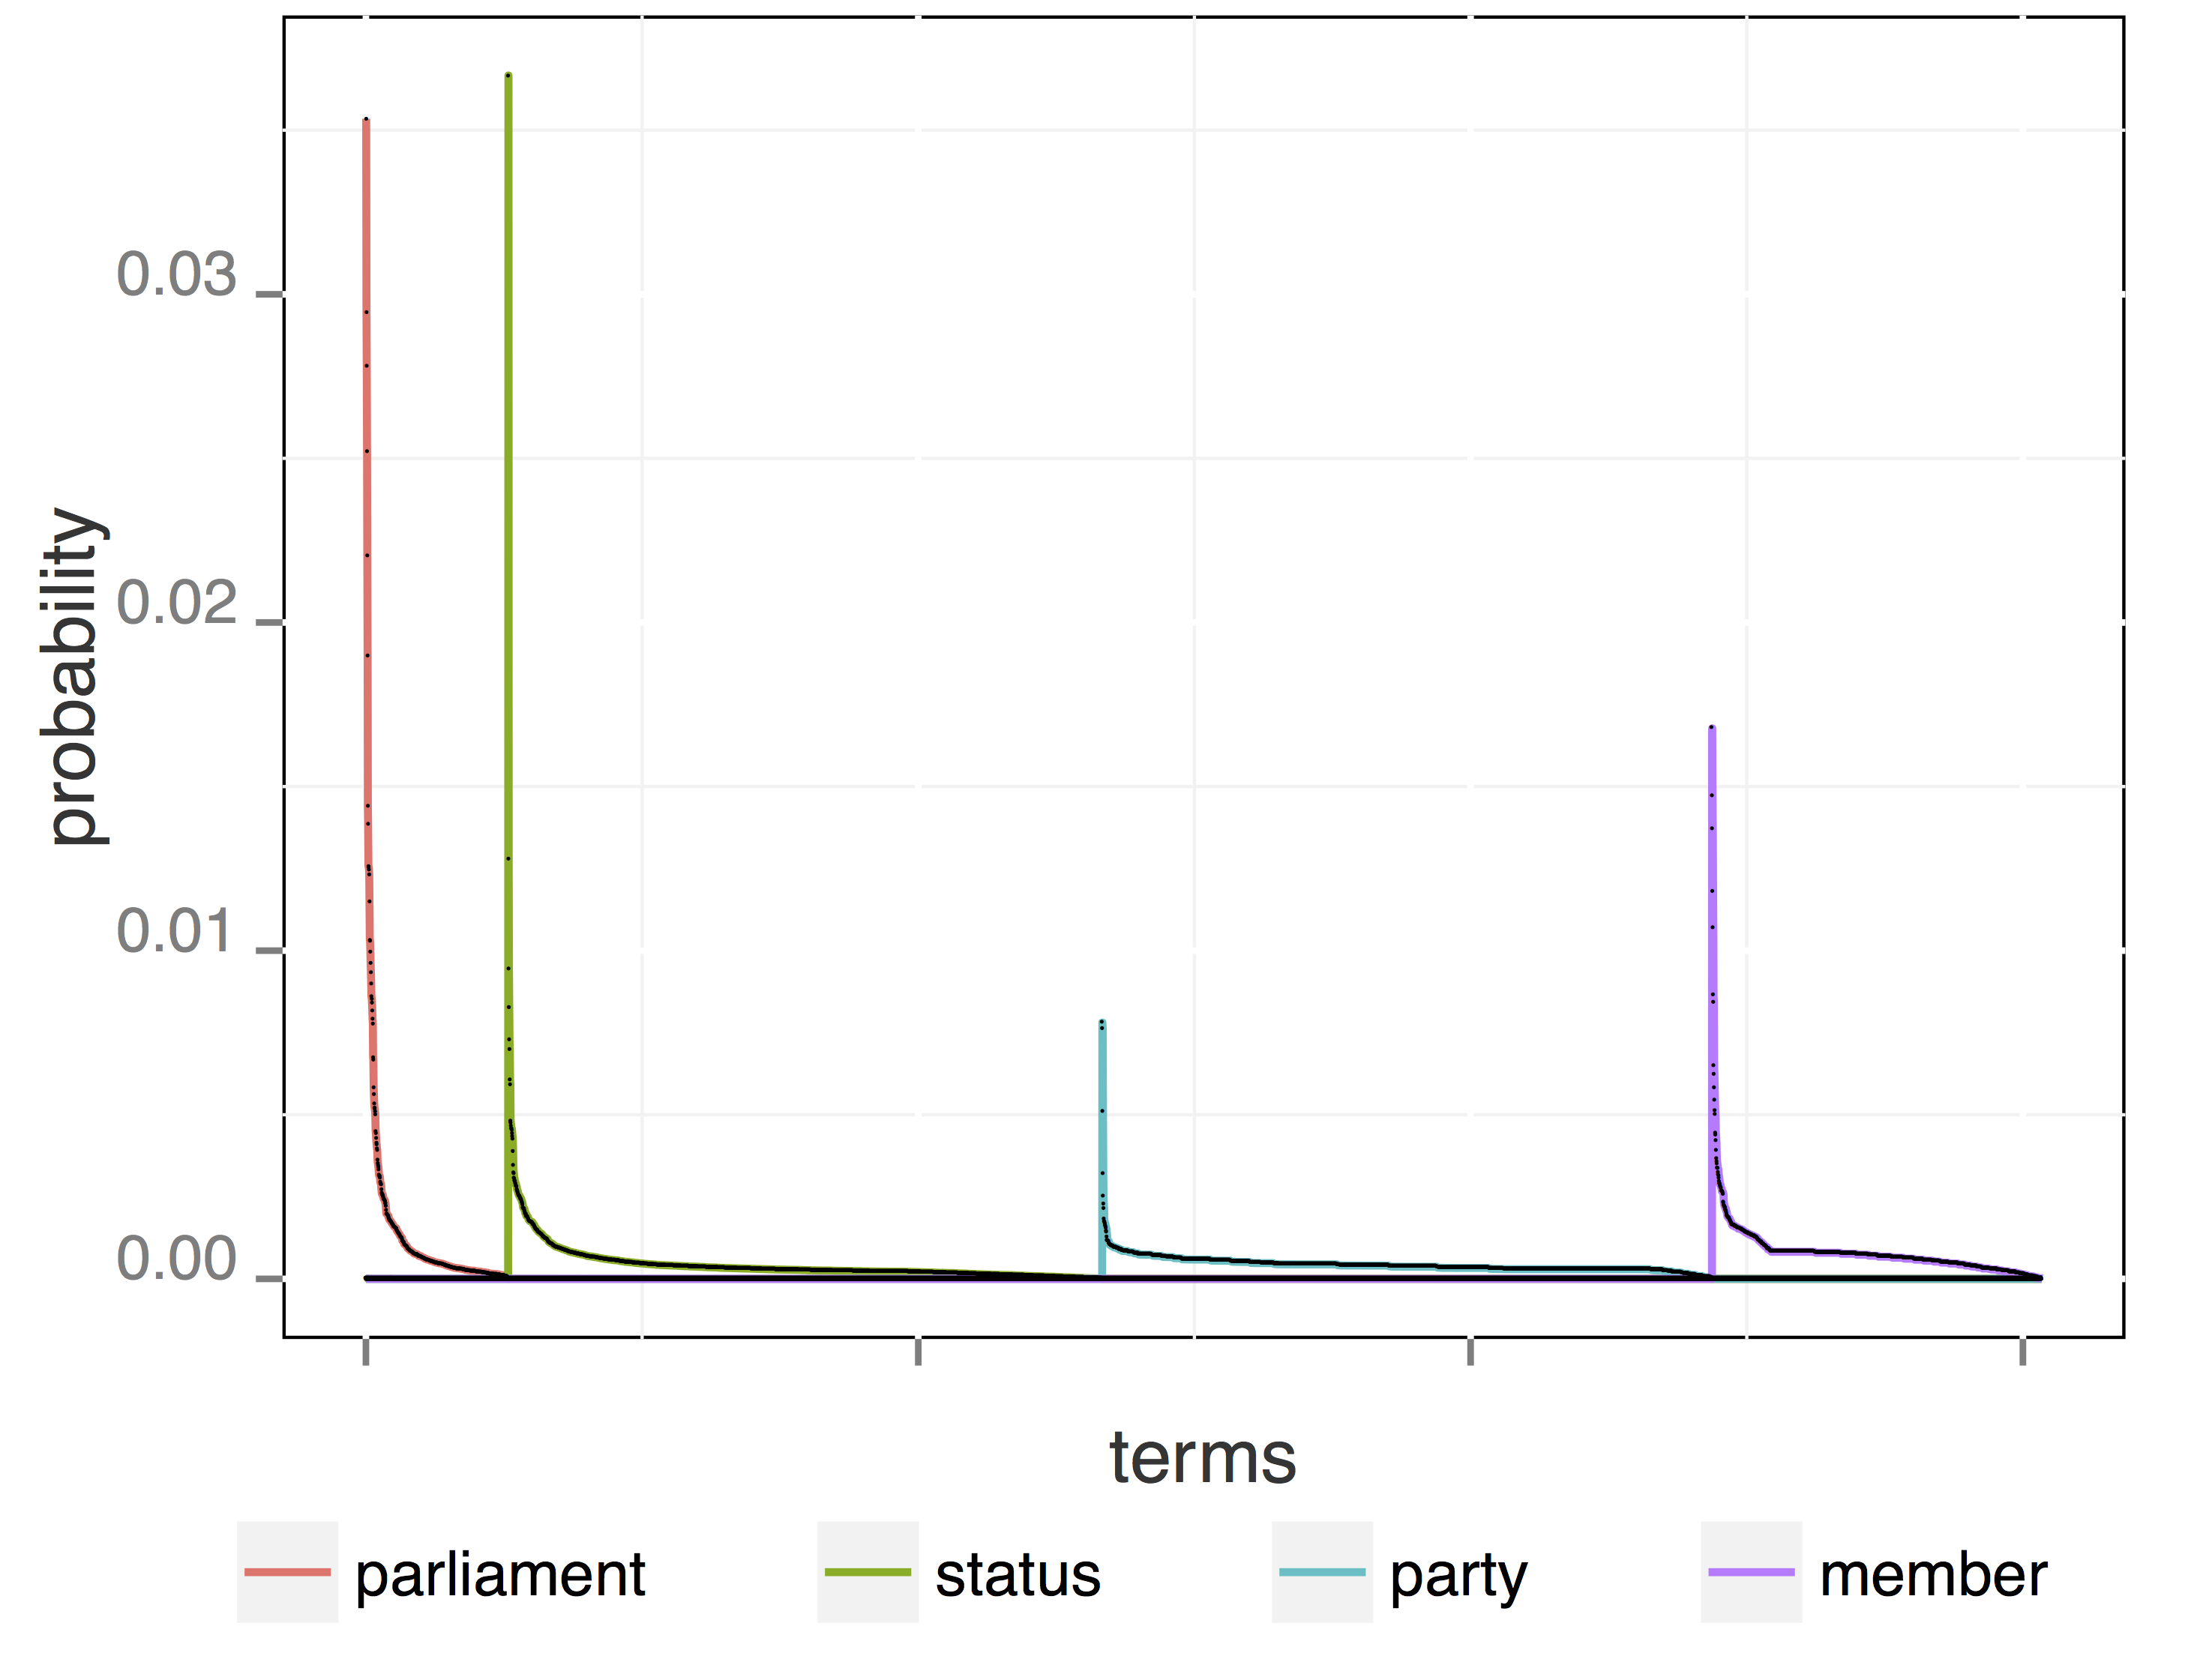
\includegraphics[width=\linewidth]{02-part-01/chapter-03/figs_and_tables/img_nlm02335.png}
\caption{\label{fig:VSC} \achswlm of D. Samson (as the member of parliament - Leader of PvdA), Labour Party (as the party), Government (as the status), and the Parliament}
        \end{subfigure}
        \caption{\label{fig:VS} \emph{Vertical Separability}: probability distribution over terms in different layers based on \hswlms in complete paths from the root to the terminal entities in the hierarchy}
\end{figure}

Two\:-\:dimensional separation property of \achswlm in the hierarchy is essentially due to the parsimonization effect in two directions. 
Intuitively, the horizontal separability is mainly the result of the specification stage. For example, when an entity is parsimonized given its direct parent, since the data in its parent is formed by pooling the data from the entity and its siblings, parsimonization makes the model of the entity separable from its siblings, which provide \emph{horizontal separation} in the resulting language models. On the other hand, vertical separability is mainly due to the generalization stage (and implicitly specification). For example, when an entity is parsimonized given its children, since they are specified already, parsimonization gets rid of the specific terms of the lower layer from the entity's model.


%---------------------------------------
\subsection{Separability for Transferability}
\label{subsec:Separability}
%---------------------------------------
As an extrinsic evaluation of the \hswlms, we investigate the effectiveness of the the learned representations in a classification task in the parliamentary dataset with an evolving hierarchical structure. The task is to predict either the party that a member of the parliament belongs to, or the status of the member's party, having all the speeches given by that member in a period,  as well as all the speeches given by the members of all parties in a different period of parliament.

In the parliament, the composition of parties and statuses changes over different periods (Figure~\ref{fig:DutchParl}) and hence the speeches related to different entities can vary dramatically.  Due to this fact, cross-period classification is notoriously challenging \citep{Hirst:2014,yu:2008}.  We show that representing entities with \achswlm tackles the problem of having non-stable models when the composition of parliament evolves during the time, by capturing the essence of language models of parliamentary entities at aggregate levels. 

We use $SVM$ as the base classifier and use the standard $SVM$ as well as a $SVM$ for training which we consider probabilities of terms in \achswlm as the weights of features in order to evaluate the effectiveness of \achswlm. Using the probabilities estimated by \achswlm as weights for features can be considered as a feature selection approach that filters out features that are not essential in accordance to the hierarchical position of entities and make the data representation more robust by taking out non-stable terms\footnote{We have also tried $SVM$ along with a feature selection methods~\citep{Forman:2003,brank:2002} that uses the Information Gain (IG) to select features as a baselines and reported the results in~\citep{Dehghani:2016:ICTIR}.}.
We have employed conventional 5-fold cross validation for training and testing and to maintain comparability, we have used the same split for folding in all the experiments.

\begin{table}[!t]
\caption{Results on the task of party classification.}
\makebox[\linewidth][c]{
\centering
\begin{subtable}[b]{0.48\textwidth}
\captionof{table}{\label{tbl:SVM-party}Accuracy of the SVM classifier.}
\begin{adjustbox}{max width=\textwidth}
\begin{tabular}{ c l l l l l} \toprule
\multicolumn{2}{ c }{\multirow{2}{*}{\textbf{Period}}} & \multicolumn{4}{ c }{\textbf{Test}}
\\  \cmidrule{3-6}
\multicolumn{1}{ c}{} & & \textit{2006-10}& \textit{2010-12}& \textit{2012-14} & \textit{All}
\\ \midrule
\multirow{4}{*}{\rotatebox[origin=c]{90}{\textbf{Train}}} & \textit{2006-10} & \tc 47.56 & 29.22 & 26.84 & -
\\  
& \textit{2010-12} & 29.87 & \tc 40.90 & 35.57 & -
\\   
& \textit{2012-14} & 31.09 & 30.51 & \tc 44.96 & -
\\   
& \textit{All} & - & - & - & \tc 39.18
\\\bottomrule
\end{tabular}
\end{adjustbox}
\shrink
\end{subtable}
%
~~
%
\begin{subtable}[b]{0.48\textwidth}
\captionof{table}{\label{tbl:swlm-party}Accuracy of the $SVM_{\achswlm}$ classifier.}
\begin{adjustbox}{max width=\textwidth}
\begin{tabular}{ c l l l l l } \toprule
\multicolumn{2}{ c }{\multirow{2}{*}{\textbf{Period}}} & \multicolumn{4}{ c }{\textbf{Test}}
\\  \cmidrule{3-6}
\multicolumn{1}{ c}{} & &2006-10&2010-12&2012-14 & All
\\ \midrule
\multirow{4}{*}{\rotatebox[origin=c]{90}{\textbf{Train}}} & 2006-10 & \tc 44.51 & 46.10 & 43.62 & -
\\  
& 2010-12 & 40.85 & \tc 40.25 & 39.59 &-
\\   
& 2012-14 & 40.24 & 38.96 & \tc 42.28 & -
\\   
& All & - & - & - & \tc 49.94
\\\bottomrule
\end{tabular}
\end{adjustbox}
\end{subtable}
}
\end{table}

\newcolumntype{Y}{>{\centering\arraybackslash}X}
\begin{table}[!t]
\fontsize{7}{8}\selectfont
%\newcolumntype{Y}{>{\centering\arraybackslash}X}
\caption{Results on the task of status classification.\vspace{-10pt}}
\makebox[\linewidth][c]{
\centering
\begin{subtable}[b]{0.5\textwidth}
\captionof{table}{\label{tbl:SVM-status}Accuracy of the $SVM$ classifier}
\begin{tabular}{ c l l l l l } 
\toprule
\multicolumn{2}{ c }{\multirow{2}{*}{\textbf{Period}}} & \multicolumn{4}{ c }{\textbf{Test}}
\\ \cmidrule{3-6}
\multicolumn{1}{ c}{} & &2006-10&2010-12&2012-14 & All
\\ \midrule
\multirow{4}{*}{\rotatebox[origin=c]{90}{\textbf{Train}}} & 2006-10 & \tc 84.14 & 68.83 & 87.24 & -
\\ 
& 2010-12 & 68.29 & \tc 78.57 & 87.91 & -
\\
& 2012-14 & 68.90 & 75.97 & \tc 88.59 & -
\\ 
& All & - & - & - & \tc 79.87
\\\bottomrule
\end{tabular}
\shrink
\end{subtable}
%
~~~
%
\begin{subtable}[b]{0.5\textwidth}
\captionof{table}{\label{tbl:swlm-status}Accuracy of the $SVM_{\achswlm}$ classifier}
\begin{tabular}{ c l l l l l } \toprule
\multicolumn{2}{ c }{\multirow{2}{*}{\textbf{Period}}} & \multicolumn{4}{ c }{\textbf{Test}}
\\  \cmidrule{3-6}
\multicolumn{1}{ c}{} & &2006-10&2010-12&2012-14 & All
\\ \midrule
\multirow{4}{*}{\rotatebox[origin=c]{90}{\textbf{Train}}} & 2006-10 & \tc 82.32 & 80.51 & 89.29 &-
\\  
& 2010-12 & 79.87 & \tc 74.66 & 88.58 &-
\\   
& 2012-14 & 78.65& 77.27 & \tc 93.28 & -
\\   
& All & - & - & - & \tc 86.98
\\\bottomrule
\end{tabular}
\end{subtable}
}
\end{table}


Tables~\ref{tbl:swlm-status} and~\ref{tbl:swlm-party} show the performance of employing \acswlm on status and party classification respectively. 
Tables~\ref{tbl:SVM-status} and~\ref{tbl:SVM-party} indicate the results of SVM classifier on status and party classification respectively. Comparing the results in Tables~\ref{tbl:swlm-status} and~\ref{tbl:SVM-status}, we see that the accuracy of SVM in within period experiments is sometimes slightly better, but in cross period experiments, the classifier which uses \acswlm of statuses achieves better results.  This is also observed in the results in Table~\ref{tbl:swlm-party} compare to the results in Table~\ref{tbl:SVM-party}. 
%

For party classification, employing \acswlm results in a more significant improvement over the baseline.  \citet{Hirst:2014} discuss that since the status of members in parliament, compared to their party, has more effect on the content of their speeches, classifiers tend to pick features related to the status, not the party ideologies. So, SVM performs very well in terms of accuracy in the within-period experiments, but this performance is indebted to the separability of parties due to their status. Hence, changing the status in cross period experiments, using the trained model on other periods fails to predict the party, so the accuracies drop down. This is exactly the point which the strength of our proposed method kicks in. 
Since for each party, the \acswlm is less affected by the status of the party in that period, the model remains valid even when the status is changed.  In other words, eliminating the effect of the status layer in the party model in the specification stage ensures that the party model captures the essential terms related to the party ideology, not its status. Thereby, it is a stable model which is transferable through the time.
%
We conducted the one-tailed t-test on the results. In both party and status classification, in all cases which \acswlm\ performs better than the SVM, the improvement is statistically significant ({p-value} $<$ 0.005).

To get a better intuition of the procedure of estimating \acswlm, consider the hierarchical relations of Dutch parliaments in the period of \emph{2006-2010} which is depicted in Figure~\ref{fig:DutchParl}. 
%
Assume that the goal is modeling language usage of ``Christian-Union (CU)'' as an entity in the party layer. In the speeches from the members of this party, words like ``\emph{Chairman}" or ``\emph{Agree}'' might occur repeatedly. However, they are not a good point of reference for the party's ideological language usage. In the procedure of estimating \acswlm\ of the "Christian-Union", these words are removed from the initial estimated standard language model in the specification stages, since ``\emph{Chairman}" is a general term in the parliamentary domain and is only able to explain the root entity and ``\emph{Agree}' is somehow an indicator of language usage of all the ``Government'' parties.
%
On the other side, consider the goal is to model language usage of ``Government'' as an entity in the status layer. Speeches from ``Christian-Union'' members, which are also counted as ``Government'' members, may contain words like ``\emph{Bible}'' or ``\emph{Charity}''.  It is trivial that involving these party-specific words in the constructed model for the ``Government'' in an individual period demolishes the comprehensiveness. In the procedure of estimating \acswlm\ for the ``Government'', in the generalization stages, these words are discarded from the model. This way, ``Government'' model does not lose its validity on other periods where the ``Christian-Union" is not in a Government party.

As another indicator of the effectiveness of \acswlm, it outperforms the SVM bringing all the data together from three different periods in both party and status classification. This is because it gets the chance of having richer train data which leads to more precise models. While in SVM, changes in the parliamentary composition make speeches diverse, and this makes it not to be able to learn a concrete model. 
\subsection{Invariance of the Representations}
\begin{figure}[!t]
\centering
\resizebox{0.9\linewidth}{!}{%
\begin{tikzpicture}
\pgfkeys{
     /pgf/number format/precision=2, 
    /pgf/number format/fixed zerofill=true,
    /pgf/number format/fixed
}
\begin{axis}[
    width= 12cm, %\textwidth,
    height=5cm, %5cm,
    ybar,%=0pt,
    ymajorgrids,
    minor tick num=1,
    bar width= 6.5pt,
    enlarge y limits=0.25,
    symbolic x coords={
    VVD,
    PvdA,
    CDA,
    PVV,
    SP,
    D66,
    CU,
    GL,
    Opposition,
    Government
},
    x tick label style={rotate=45,anchor=east},
    xtick=data,
    % ymin=0.0, 
    % ymax=0.5,
    ytick = {0.00,0.10,0.20,0.30,0.40,0.50},
    ylabel={},
    %legend style={at={(0.9,0.95),font=\fontsize{5}{6}},
    anchor=north,
    ylabel={JS-Divergence},
%    legend style={at={(0.65,-0.2),font=\fontsize{5}{6}},
    legend style={at={(0.965,0.95),font=\fontsize{5}{6}\selectfont},
    legend columns=1
    },
    nodes near coords,
    every node near coord/.append style={font=\fontsize{3}{4}\selectfont, rotate=90, anchor=west},
    %nodes near coords align={vertical},
    tick label style={font=\fontsize{5}{6}\selectfont}
    ]
\definecolor{b}{HTML}{3399FF}
\definecolor{g}{HTML}{5C7C19}
\addplot[fill=b, draw=b] coordinates
{
(VVD,0.3422)
(PvdA,0.3917)
(CDA,0.3889)
(PVV,0.2422)
(SP,0.3050)
(D66,0.2979)
(CU,0.4336)
(GL,0.4471)
(Opposition,0.1562)
(Government,0.2471)
};

\addplot[fill=g, draw=g, pattern color = g, pattern = north west lines] coordinates
{
(VVD,0.1639)
(PvdA,0.1631)
(CDA,0.1666)
(PVV,0.1641)
(SP,0.1918)
(D66,0.1890)
(CU,0.1757)
(GL,0.2759)
(Opposition,0.0512)
(Government,0.0759)
};

\legend{SLM,\acswlm}

\end{axis}
\end{tikzpicture}
}
\vspace{-12pt}
\caption{
Average of JS-Divergence of standard language models and {\acswlm}s for parliamentary entities in three different periods.\label{fig:cross_period_party_rep_divergence}}
 \vspace{-10pt}
 \end{figure}

As an intrinsic evaluation of the models, we evaluate the invariance of representations learned by our model over different periods\:---\:how similar are models of a particular in the hierarchy when trained on data from different periods. 
%
Since \achswlm is supposed to capture the essence of entities, not only \achswlm of an entity learned using an individual period should be valid for representing the entity on other periods, but also models of the same entity learned on data from different periods should be invariant. 

To assess this, we use the diversity of entities' models in different periods to measure their (in)variance over time.
%
First, all \achswlm from different periods of each party and each status is smoothed using Jelinek-Mercer smoothing \citep{Zhai:2001} considering all parliamentary speeches in the corresponding period as the background collection and with the same value of the smoothing parameter. Then, we use the Jensen-Shannon divergence as the diversity metric to measure dissimilarities between each two {\achswlm}s learned from different periods and then calculate the average of values for each entity. As the baseline, the same calculation is done for the standard language models of entities, i.e., language models estimated using maximum likelihood estimation. 
Figure~\ref{fig:cross_period_party_rep_divergence} shows the diversity of models in different periods.
%
As can be seen, in all entities in both party and status layers, diversity of \achswlm of different periods is lower than diversity of standard language models, which shows the extracted {\achswlm}s are more invariant over different periods. 


In order to better understand the results in the previous section, we zoomed in on the period of 2010-12 and 2012-2014 and looked into the confusion matrices of cross-period experiments and observed that most of the errors made by $SVM$ are misclassifying members of CDA to PvdA and vice versa. These are the two parties that their statuses have been changed in these periods.  

\pgfplotstableread{
0    0.4801  0.8616  0.7492  
1    0.5667  0.5941  0.2422
2    0.3422  0.3222  0.6822
}\dataset

\definecolor{b}{HTML}{4981CE}
\definecolor{g}{HTML}{859C27}
\definecolor{r}{HTML}{B22222}
\definecolor{o}{HTML}{FF6600}

\begin{figure}[t]
\centering
\begin{tikzpicture}
\pgfkeys{
    /pgf/number format/precision=2, 
    /pgf/number format/fixed zerofill=true,
    /pgf/number format/fixed
}
\begin{axis}[
    width= 8.4cm, %\textwidth,
    height=5.7cm, %5cm,
    enlarge y limits=0.0,
    enlarge x limits=0.2,
    ymajorgrids,
    minor tick num=1,
    ybar,%=0pt,,
    bar width= 12pt,
    xtick=data,
    xticklabel style = {font=\fontsize{7}{8}\selectfont, align=center, text width=1.8cm},
    xticklabels = {Different Parties Same Period, Same Party Different Periods, Different Parties  Different Periods},
    ymin=0.0, 
    ymax=1.0,
    ytick = {0.00,0.10,0.20,0.30,0.40,0.50,0.60,0.70,0.80,0.90, 1.0},
    label style = {font=\fontsize{7}{8}\selectfont, yshift=0.5ex},
    anchor=north,
    ylabel={JS-Divergence},
    legend style={at={(0.965,0.95),font=\fontsize{5}{6}\selectfont},
    legend columns=-1
    },
    nodes near coords,
    every node near coord/.append style={font=\fontsize{5}{6}\selectfont, rotate=90, anchor=west},
    tick label style={font=\tiny},
    ]

\addplot[fill=b, draw=b, pattern color = b, pattern = north east lines] table[x index=0,y index=1] \dataset; 

\addplot[fill=r, draw=r, pattern color = r, pattern = dots] table[x index=0,y index=3] \dataset; 

\legend{TF,\achswlm}

\end{axis}
\end{tikzpicture}
\caption{
Average diversity of the representation of features of CDA and PvdA in different situations.}
\label{fig:cross_period_rep_divergence}
 \end{figure}

We investigate representations of these two parties to understand how separation in the feature representation affects the performance of cross period classification. To do so, for each of these two classes, in each period, we extract three probability distributions on terms indicating their importance based on different weighting approaches: 1) Term Frequency (used as feature weights in $SVM$) and 2) probability of terms in \achswlm (used as feature weights in $SVM_{\achswlm}$). 
Then, as a metric to measure separability of features, we use the Jensen-Shannon divergence to calculate diversity of probability distributions in three cases: 1) Different Parties in the Same Period, 2) Same Party in Different Periods 3) Different Parties in Different Periods. 
To avoid the effect of the number of features on the value of divergence, we take the top 500 high scored terms of each of the weighting methods as the fixed length representatives of them. Figure~\ref{fig:cross_period_rep_divergence} shows the average diversity of distributions in each of the three cases for each of the three weighting methods.

As expected, the diversity of features for different parties in a same period is high for both methods. However, when we calculate the diversity of features for a same party in different periods, feature representations are different in  $TF$, which causes false negative errors in the classification of these two parties. An interesting observation is in the case of having different parties in different periods, while we have two different parties their feature representations are similar in $TF$, which leads to false positive errors in the classification. 

Considering these observations together reveals that $SVM$ learns representations on the basis of features that are indicators of issues related to the status of parties, since they are the most discriminating terms considering one period and in within period experiments, the performance of $SVM$ is indebted to the separability of parties based on their statuses. Hence, after changing the status in the cross period experiments, the trained model of the previous period generated by $SVM$ fails to predict the accurate party.  In the same way, the status classifier is affected by different parties forming a government in different periods, leading to lower accuracies.   

This is exactly the point which the strengths of \achswlm kicks in. In fact, two\:-\:dimensional separability in the feature representation, enables $SVM_{\achswlm}$ to tackle the problem of having non-stable features in the model when the status of a party changes over time. In other words, eliminating the effect of the status layer in the party model, which is the result of the horizontal separation, ensures that the party model captures the terms related to the party ideology, not its status. Thereby, not only $SVM_{\achswlm}$ learns an effective model with acceptable accuracy in within period experiments, but also its learned models remain valid when the statuses of parties change. 
